\documentclass[12pt]{article}
\usepackage{a4}
\usepackage[english]{babel}
\setlength{\parindent}{0.35cm}
\pagestyle{headings}
\usepackage{graphicx}
\usepackage{grffile}
%Multiple picture in one figure
%\usepackage{subfigure}
\usepackage{subfig}
\usepackage[utf8]{inputenc}
\usepackage{listings}
\usepackage{color}
\usepackage{wrapfig}
%Floating-Umgebungen
\usepackage{float}
%Math-Environment
\usepackage{amsmath}
\usepackage{amssymb}
%Better SI-Units
\usepackage{siunitx}
%Using Appendix
\usepackage[title]{appendix}
%Using URL
\usepackage[hidelinks]{hyperref}
%Using Colored Tables
\usepackage{colortbl}
\newcommand{\gray}{\rowcolor[gray]{.90}}
\usepackage{esvect}
% Use fancy tables
\usepackage{tabularx}
% Build fancy tables
\usepackage{booktabs}
%Configure geometry
\usepackage{geometry}
\geometry{
	a4paper,
	left=3cm,
	right=3cm,
	top=3cm,
	bottom = 3cm,
	}

\lstset{
	language=C++,
	basicstyle=\small\ttfamily,
	keywordstyle=\color{blue}\ttfamily,
	stringstyle=\color{red}\ttfamily,
	commentstyle=\color{green}\ttfamily,
	morecomment=[l][\color{magenta}]{\#},
}


\usepackage{amsthm}

\renewcommand\qedsymbol{$\blacksquare$}
\newtheorem{theorem}{Theorem}[section]

\begin{document}
	
	\title{
		\textbf{\huge{CSE 446: Machine Learning Winter 2018 }} \\[2cm]
		\LARGE{Assignment 2}\\[1cm]
	}
	\author{from \\ Lukas Nies \\ University of Washington}
	\date{02/01/18}
	\clearpage\maketitle\thispagestyle{empty}
	\newpage

	\tableofcontents
	\setcounter{page}{0}
	\newpage
	
	% To start with section 1 labeled as section 0
	\setcounter{section}{-1}
	

\section{Policies}

\subsection{List of Collaborators}

My collaborator was Edith Heiter (discussed Problem 2 and 4). The development of the answers though was completely independent and individually.

\subsection{List of Acknowledgments}

None.

\subsection{Policies}

I have read and understood these policies.

\section{Perceptron Exercise}

The evolution of the weight vector $w$ are shown in figure \ref{fig:1.1} after the data was observed so the weights were already updated. In the same figure the maximum margin is shown since the perceptron didn't maximize the margin after the training set.

\begin{figure}[b!]
	\centering
	\subfloat[Step One] {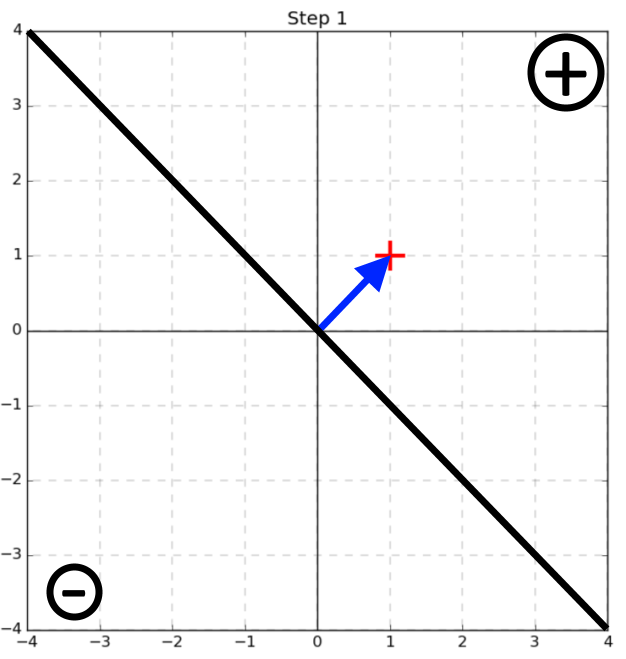
\includegraphics[width=0.24\textwidth]{../Problem_1/step_1.png}}
	\hfill
	\subfloat[Step Two] {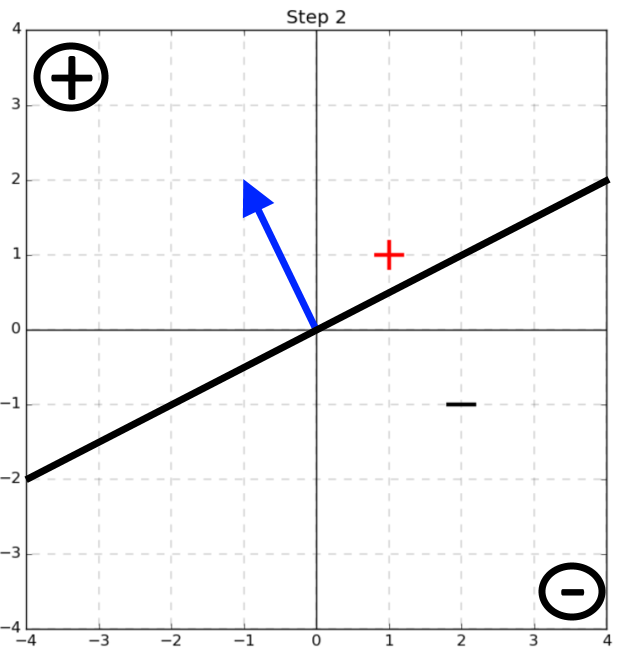
\includegraphics[width=0.24\textwidth]{../Problem_1/step_2.png}}
	\hfill
	\subfloat[Step Three] {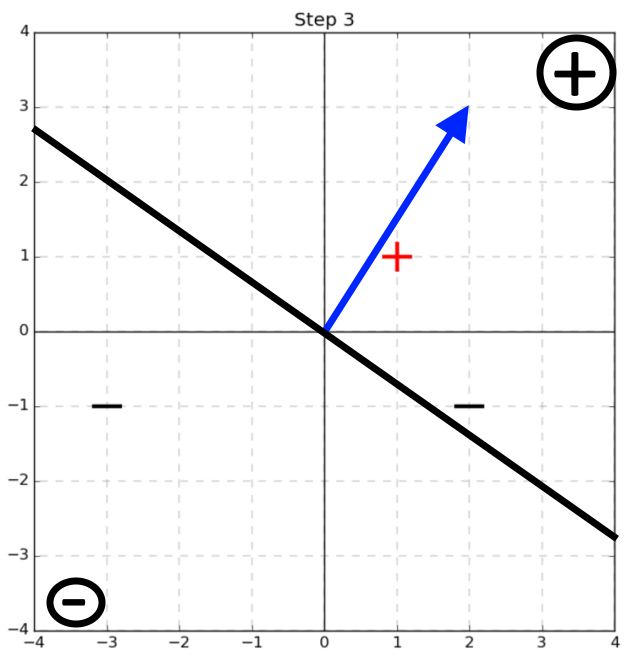
\includegraphics[width=0.24\textwidth]{../Problem_1/step_3.png}}
	\hfill
	\subfloat[Step Four] {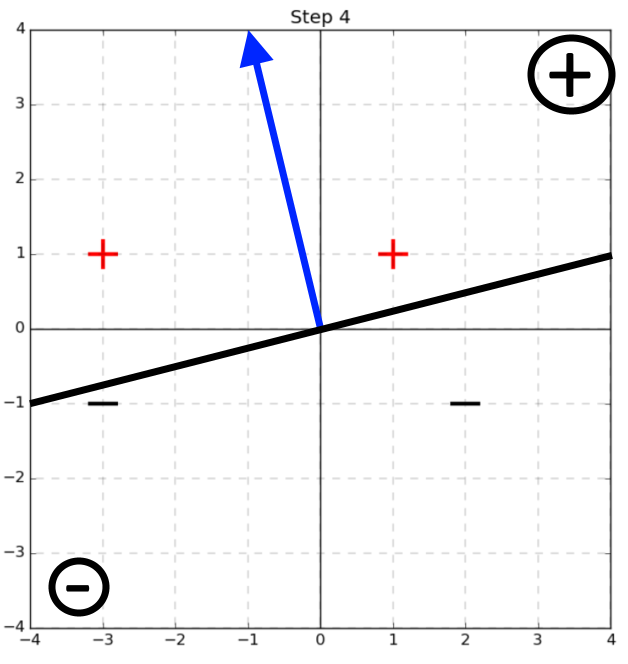
\includegraphics[width=0.24\textwidth]{../Problem_1/step_4.png}}
	\hfill
	\subfloat[Maximum margin] {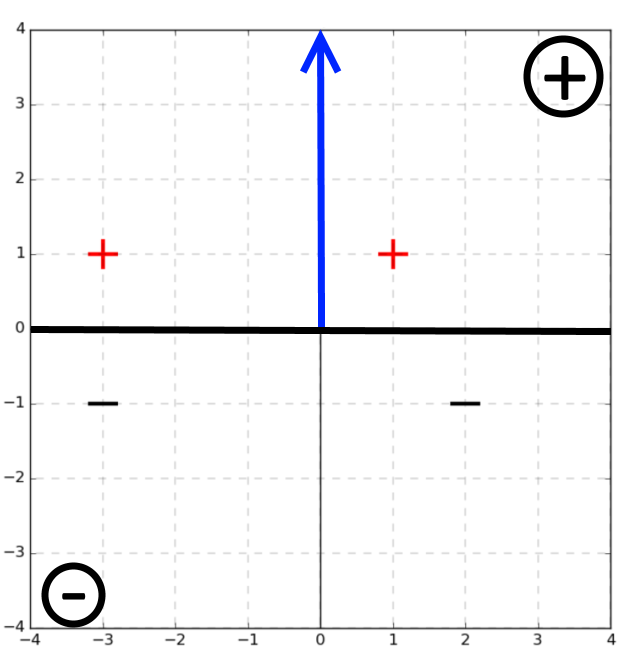
\includegraphics[width=0.24\textwidth]{../Problem_1/opt.png}}
	\caption[]{Visualization of the perceptron's decision boundary. The plots show the weight vector $w$ in blue  and the corresponding decision boundary (black) after they were updated. Plot (e) shows the maximum decision margin which is has the value $1$ in this case. }
	\label{fig:1.1}
\end{figure}
\noindent
To solve Problem 1.3 I will follow the proof according to \cite{CIML}. 
\begin{theorem}
	If data $D$ is linear separable with the geometric margin $\gamma^* = 0.5$ and has the maximum norm $\lVert x \rVert\leq 5 \forall x \in D$ then the algorithm will convert after at most $\frac{25}{\gamma^2}$ updates. 
\end{theorem}
\begin{proof}
	Suppose $x^*$ realizes $\gamma^*>0$ and let $w^{(k)}$ be the $k^{th}$ weight vector after $k$ updates. We show in the following that the angle between $w$ and $w^*$ decreases such that the algorithm converges. That is when $w^*\cdot w$ increases faster than $\lVert w \rVert^2$.\\
	After the $k^{th}$ update we find
	\begin{align*}
		w^*\cdot w^{(k)} = w^{*}\left( w^{(k-1)}+yx \right) = w*\cdot w^{(k-1)} + yw^*\cdot x \geq w*\cdot w^{(k-1)} + k\gamma 
	\end{align*}
	and
	\begin{align*}
		\lVert w^{(k)} \rVert^2=\lVert w^{(k-1)} + yx \rVert^2 = \lVert w^{(k-1)} \rVert^2 + 2yw^{(k-1)}\cdot x + y^2\cdot\lVert x \rVert^2 \geq \lVert w^{(k-1)} \rVert^2 +5^2 +0
	\end{align*}
	The last line shows that $\lVert w^{(k)} \rVert$ increases by at least $25$ every update. Therefore $\lVert w^{(k)} \rVert^2 \leq 25k$. So
	\begin{align*}
	\sqrt{25k} \geq \lVert w^{(k)} \rVert \geq w^*\cdot w^{(k)} \geq 5\gamma \Leftrightarrow k \leq \frac{25}{\gamma^2}
	\end{align*}
\end{proof}
\noindent
The maximum number of mistakes (updates) the perceptron has to make until it converges is given by $\frac{25}{\gamma^2}=\frac{25}{0.25}=100$.

\newpage

\section{Implementation: Perceptron}

See tables \ref{tab:1} and \ref{tab:2} for answers to questions 2 to 5. Some interesting plots concerning question 1 to 5 are shown in figure \ref{fig:2.close}. 
Some remarks to the implementation: the implemented algorithm takes the number of iterations and the filenames from the command line and then loops for a certain amount of iterations over the perceptron and trains the weight vector. If the algorithm converges, a lower bound is calculated as the smallest normalized weight vector encountered in the training process. At 10\% and 90\% of the epochs the weight vector is printed to check whether some features might be noise or not. In order to create a development set, the training set was split into 4:1, generating a tuning set of 200 examples to tune the maximal number of iterations. This hyper parameter was achieved by training the perceptron and then testing with the development set for the lowest development error. The corresponding number of epochs was chosen to test calculate the training, development and test error. Plots will be saved for a general overview of the results. \par 
To tune the performance on set 6 I merged training set 6, 7, and 8 to create a larger training set and deleted some features I expected to be noise (see figure \ref{fig:2.1.surprise}).

\begin{figure}[b!]
	\centering
	\subfloat[Set 2] {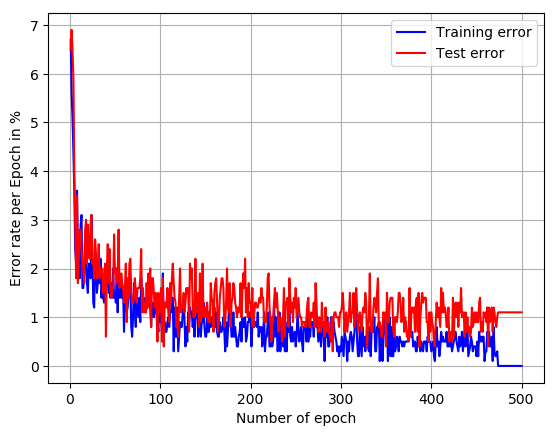
\includegraphics[width=0.24\textwidth]{../Problem_2/A2.2.train.tsv.full.png}}
	\hfill
	\subfloat[Set 3] {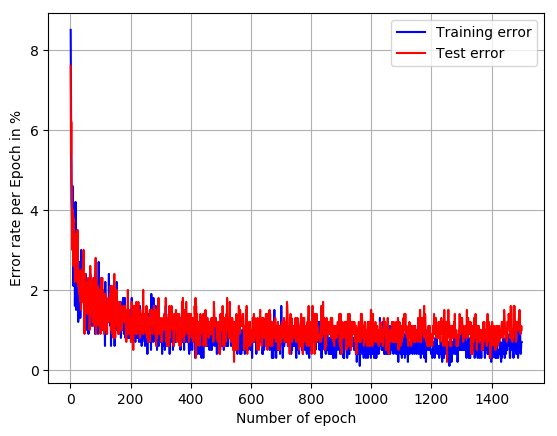
\includegraphics[width=0.24\textwidth]{../Problem_2/A2.3.train.tsv.full.png}}
	\hfill
	\subfloat[Set 4] {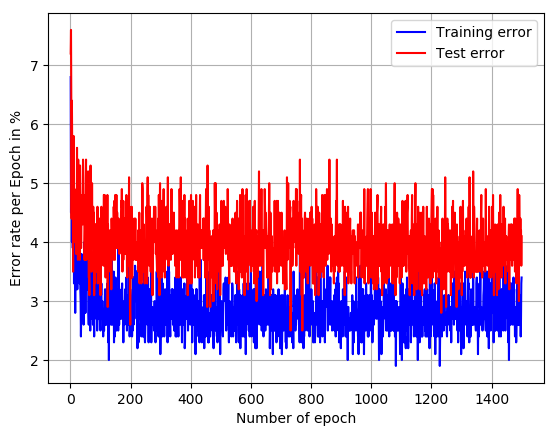
\includegraphics[width=0.24\textwidth]{../Problem_2/A2.4.train.tsv.full.png}}
	\hfill
	\subfloat[Set 5] {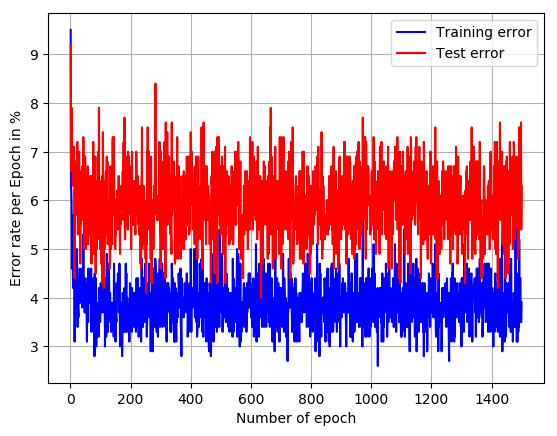
\includegraphics[width=0.24\textwidth]{../Problem_2/A2.5.train.tsv.full.png}}
	\hfill
	\subfloat[Set 6] {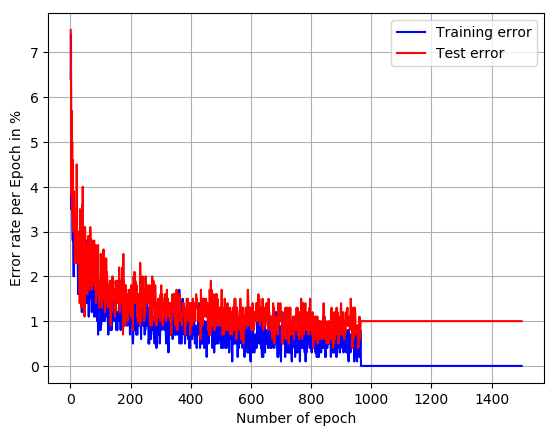
\includegraphics[width=0.24\textwidth]{../Problem_2/A2.6.train.tsv.full.png}}
	\hfill
	\subfloat[Set 7] {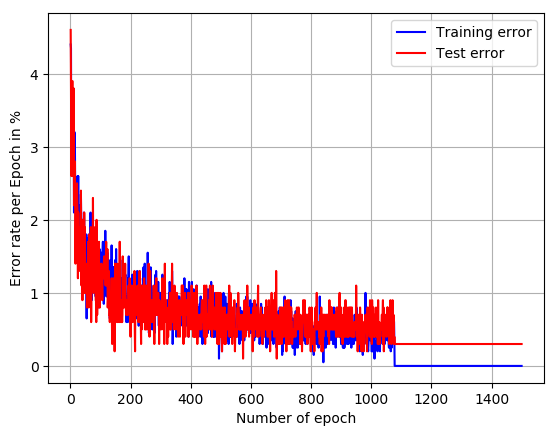
\includegraphics[width=0.24\textwidth]{../Problem_2/A2.7.train.tsv.full.png}}
	\hfill
	\subfloat[Set 8] {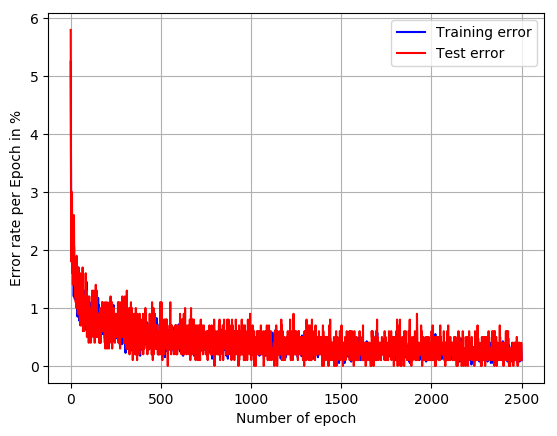
\includegraphics[width=0.24\textwidth]{../Problem_2/A2.8.train.tsv.full.png}}
	\hfill
	\subfloat[Set 9] {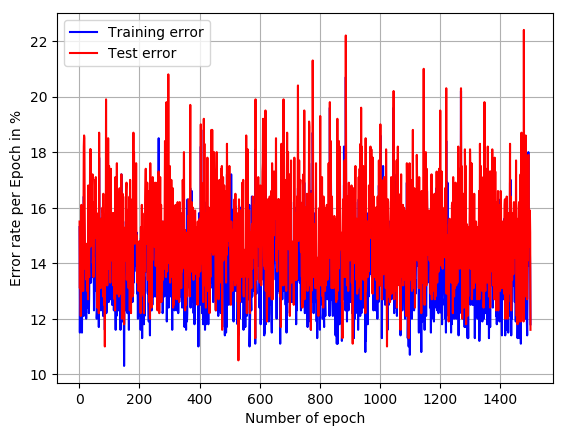
\includegraphics[width=0.24\textwidth]{../Problem_2/A2.9.train.tsv.full.png}}
	\caption[]{Visualization of the error rates of the different sets. In blue the training error rate and in red the test error rate. }
	\label{fig:2.1}
\end{figure}

\noindent

When looking at data 6 to 8 we can see that the data is from the same source and not overlapping. In order to increase the precision on the test set (which is the same for 6 to 8) we merged the three training data sets combining now a total of 7000 observations to train the perceptron and do nt consider the features which we expect to me noise (in this case, feature 10, 12, and 18). The result can be seen in table \ref{tab:3} and figure \ref{fig:2.1.surprise} and \ref{fig:2.close}.

% Table generated by Excel2LaTeX from sheet 'Sheet1'
\begin{table}[H]
	\centering
	\begin{tabularx}{\textwidth}{c|X|X|X|X|}
		& \multicolumn{4}{c|}{question number} \\
		dataset & \multicolumn{1}{c}{2} & \multicolumn{1}{c}{3} & \multicolumn{1}{c}{4} & \multicolumn{1}{c|}{5} \\
		\midrule
		2     &   Is linear separable because error rates don't change after $\approx 380$ epochs, the smallest margin found is $\approx 0.005$, see figure \ref{fig:2.1}(a)  &  Does overfit slightly since test set error rises slowly for longer training times, see \ref{fig:2.1}(a) and doesn't match the trainings error     &   Weight of feature 9 is one to two orders of magnitude smaller than the others, might be noise  & Tuned maximum number of iterations, set it to $94$, got $8\%$ training error, $19\%$ test error, $4\%$ development error \\
		\midrule
		3     &   Is not linear separable because it does not converge and error rate rises a little after $\approx 1500$ epochs    &    Does overfit a little, see figure \ref{fig:2.1}(b) since test error rises with growing numbers of epochs   &   Weight of feature 6 and 19 are one to two orders of magnitude smaller than the others, might be noise    & Tuned maximum number of iterations, set it to $176$, got $10\%$ training error, $10\%$ test error, $3\%$ development error \\
		\midrule
		4     &   Is not linear separable because it does not converge and error rate rises a little after $\approx 1500$ epochs, doesn't match the training error, see figure \ref{fig:2.1}(c)   &    Does overfit strongly training and test error don't fit at all   &   No obvious noise found    & Tuned maximum number of iterations, set it to $815$, got $20\%$ training error, $46\%$ test error, $7\%$ development error (overall bad performance) \\
		\midrule
		5     &   Is not linear separable because it does not converge and test error is steadily above training error rate     &    Does overfit strongly, errors don't match at all, see plot \ref{fig:2.1}(d)   &   No obvious noise found    & Tuned maximum number of iterations, set it to $632$, got $17\%$ training error, $31\%$ test error, $8\%$ development error (overall bad performance) \\
		\bottomrule
	\end{tabularx}%
	\caption{Tabel with answers to questions of problem 2.}
	\label{tab:1}%
\end{table}%

% Table generated by Excel2LaTeX from sheet 'Sheet1'
\begin{table}[H]
	\centering
	\begin{tabularx}{\textwidth}{c|X|X|X|X|}
		& \multicolumn{4}{c|}{question number} \\
		dataset & \multicolumn{1}{c}{2} & \multicolumn{1}{c}{3} & \multicolumn{1}{c}{4} & \multicolumn{1}{c|}{5} \\
		\midrule
		6     &   The data is linear separable since the algorithm converges after roughly $\approx 1210$ epochs, the smallest margin is $\approx 0.004$     &    Does overfit slightly for larger epochs (see figure \ref{fig:2.1}(e)) since test error is larger than training error   &   Feature 12 generates a weight which is 3 orders of magnitude smaller then the others, this might be noise    & Tuned maximum number of iterations, set it to $68$, got $13\%$ training error, $28\%$ test error, $4\%$ development error \\
		\midrule
		7     &   The data is linear separable since the algorithm converges after roughly $\approx 1300$ epochs,  the smallest margin is $\approx 0.005$    &    Does not overfit for larger epochs (see plot \ref{fig:2.1}(f)) since error rates are not separable   &   Feature 10, 12 and 18 generate weights which are 3 to 4 orders of magnitude smaller then the others, this might be noise    & Tuned maximum number of iterations, set it to $224$, got $6\%$ training error, $6\%$ test error, $3\%$ development error \\
		\midrule
		8     &   The data is linear separable since the algorithm converges after roughly $\approx 1300$ epochs,  the smallest margin is $\approx 0.005$    &    Does not overfit, test error is nearly identical with training error, see plot \ref{fig:2.1}(g)   &   Feature 10, 12 and 18 still generate weights which are 3 to 4 orders of magnitude smaller then the others, this might be noise    & Tuned maximum number of iterations, set it to $806$, got $8\%$ training error, $2\%$ test error, $4\%$ development error \\
		\midrule
		9     &   Is not linear separable because it does not converge and error is nearly steady    &    Strongly overfit since test error is steadily roughly two percent worse than training error rate (see plot \ref{fig:2.1}(h))   &   Weight of feature 1 and 20 are one to two orders of magnitude smaller than the others, might be noise    & Tuned maximum number of iterations, set it to $409$, got $80\%$ training error, $154\%$ test error, $27\%$ development error (very bad performance, might not be a problem solvable by the perceptron.) \\
		\bottomrule
	\end{tabularx}%
	\caption{Continuation of the answers for the first table.}
	\label{tab:2}%
\end{table}%

\begin{table}[h!]
	\centering
	\begin{tabularx}{\textwidth}{c|X|X|X|X|}
		& \multicolumn{4}{c|}{question number} \\
		dataset & \multicolumn{1}{c}{2} & \multicolumn{1}{c}{3} & \multicolumn{1}{c}{4} & \multicolumn{1}{c|}{5} \\
		\midrule
		Surpr.     &   Should be separable since it's from the same type of data as data 6, 7, and 8, so lower limit for the margin should be similar   &  Does not overfit, test error seems to perform equally good, maybe even better than training error      &   Since the "noisy" features were not considered while training and testing, no small weights could be found & Tuned maximum number of iterations, set it to $631$, got $13\%$ training error, $2\%$ test error, $7\%$ development error \\
		\midrule
		\bottomrule
	\end{tabularx}%
	\caption{Surprising table with answers to the surprise problem.}
	\label{tab:3}%
\end{table}%

\begin{figure}[h!]
	\centering
	\subfloat[Set 5 zoomed] {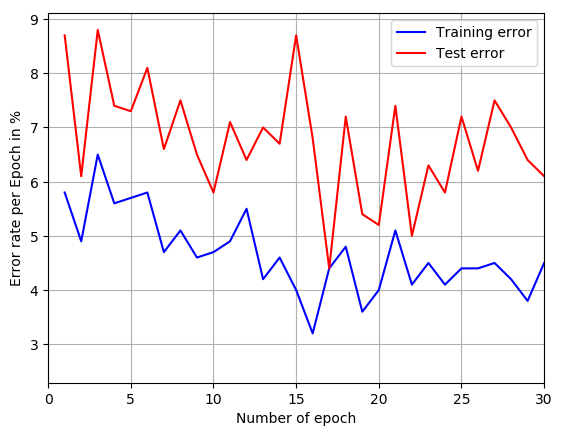
\includegraphics[width=0.24\textwidth]{../Problem_2/A2.5.train.tsv.early.png}}
	\hfill
	\subfloat[Set 10 zoomed] {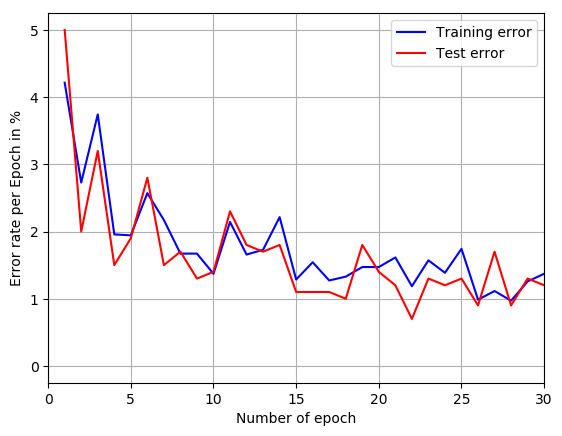
\includegraphics[width=0.24\textwidth]{../Problem_2/A2.10.train.tsv.early.png}}
	\hfill
	\subfloat[Set 10 early epoch] {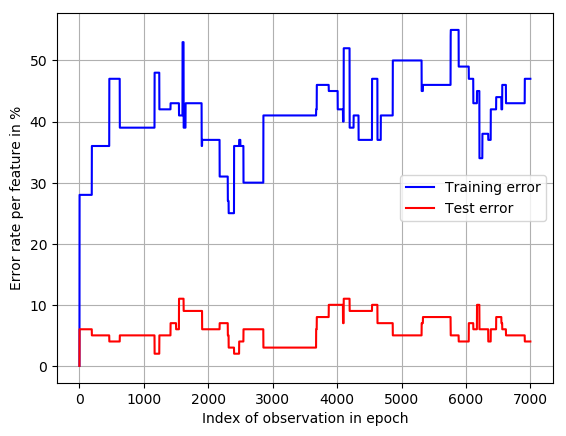
\includegraphics[width=0.24\textwidth]{../Problem_2/A2.10.train.tsv.inner_loop_at_10.png}}
	\hfill
	\subfloat[Set 10 late epoch] {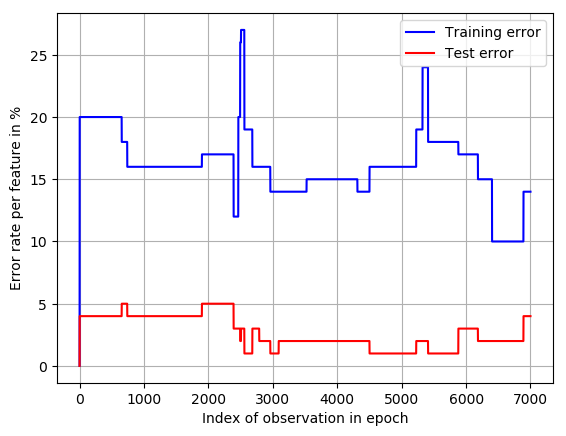
\includegraphics[width=0.24\textwidth]{../Problem_2/A2.10.train.tsv.inner_loop_at_90.png}}
	\caption[]{In (a) and (b) zoomed plots for early epochs for set 5 and 10 are shown (set 10 is set 7+8+9 - noise). We can clearly see that set 5 starts with large discrepancy between the two error rates where set 10 has good performance on both training and test rate. Plot (c) and (d) show the error rate changing after encountering new observations for an early epoch (c) and a late epoch (d) in training set 10. We can see that in late epochs less mistakes are made as in earlier epochs. }
	\label{fig:2.close}
\end{figure}

\begin{figure}[h!]
	\centering
	\subfloat[1000 datapoints] {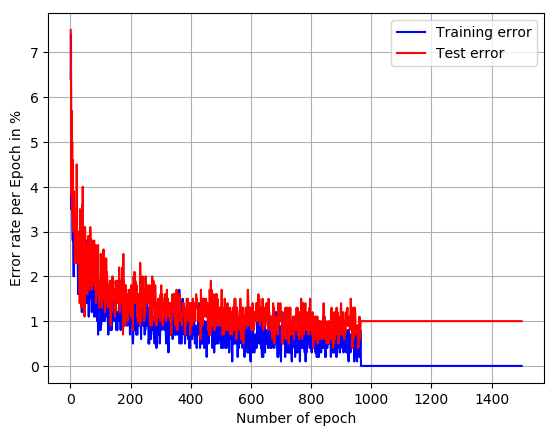
\includegraphics[width=0.24\textwidth]{../Problem_2/A2.6.train.tsv.full.png}}
	\hfill
	\subfloat[2000 datapoints] {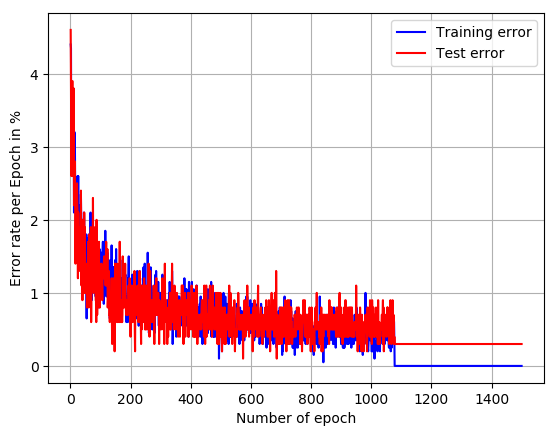
\includegraphics[width=0.24\textwidth]{../Problem_2/A2.7.train.tsv.full.png}}
	\hfill
	\subfloat[4000 datapoints] {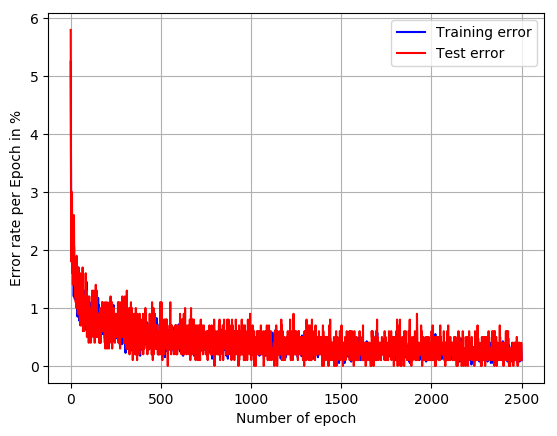
\includegraphics[width=0.24\textwidth]{../Problem_2/A2.8.train.tsv.full.png}}
	\hfill
	\subfloat[7000 datapoints and noise cancellation] {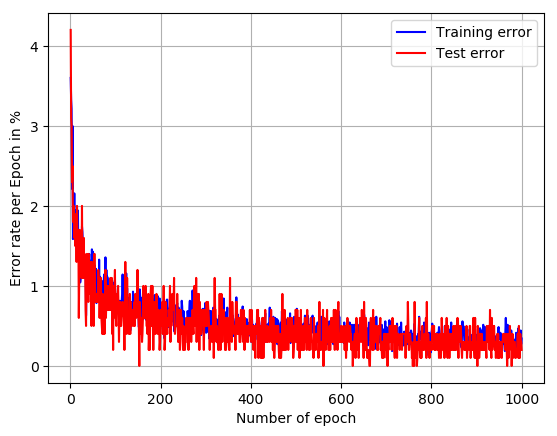
\includegraphics[width=0.24\textwidth]{../Problem_2/A2.10.train.tsv.full.png}}
	\caption[]{Visualization of the error rates of the  sets from the same source with different sizes of training data . In blue the training error rate and in red the test error rate. }
	\label{fig:2.1.surprise}
\end{figure}


\newpage

\section{Beat the Perceptron}
 
To beat the perceptron I implemented the voted perceptron approach in order to yield better results by paying with longer processing time. I focused on data set number 9 since the performance was quite bad in the normal approach and I wanted to test how strong the voted perceptron is even if the data is not linear separable. In figure \ref{fig:3.1} the results for the voted perceptron and the normal perceptron are compared.\par 
After tuning the hyperparameter of maximum interation steps for the voted perceptron I found an trainingset error of 80\%, test error of 120\% and a dev error of 40\%. By comparing both sub plots in figure \ref{fig:3.1} one can see that the overall performance is increased by nearly 5\% compared to the normal perceptron implementation. \par
Even though I didn't expect life-changing by trying to solve a not perceptron solvable problem with another perceptron implementation (not linear separable!) I achieve a quite good improvement in the performance. 

 
\begin{figure}[h!]
 	\centering
 	\subfloat[Perceptron on set 9] {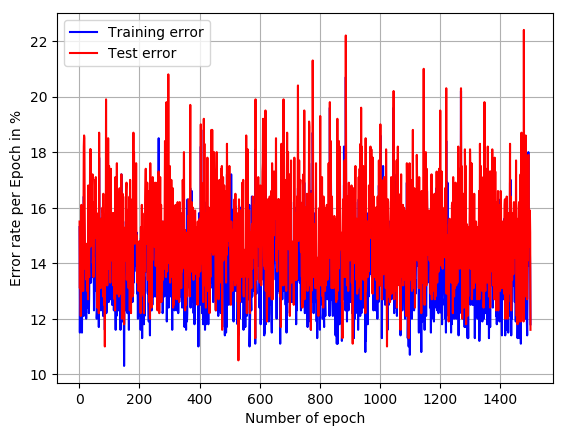
\includegraphics[width=0.49\textwidth]{../Problem_2/A2.9.train.tsv.full.png}}
 	\hfill
 	\subfloat[Voted perceptron on set 9] {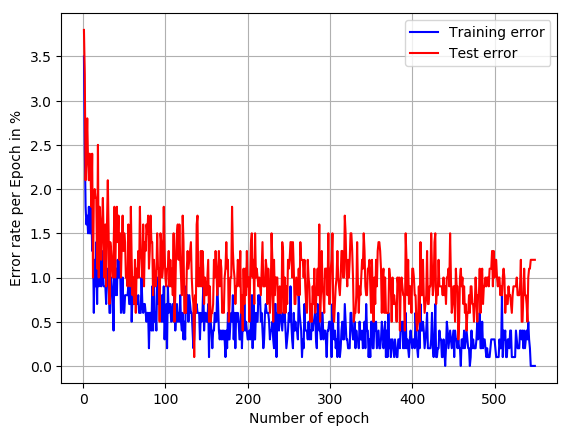
\includegraphics[width=0.49\textwidth]{../Problem_2/A2.11.train.tsv.full.png}}
 	\caption[]{Visualization of the error rates of set 9 when treated by perceptron (left) and voted perceptron (right). }
 	\label{fig:3.1}
\end{figure}
 
\newpage


\section{PCA on Digits}

\subsection{Convariance matrix construction}

Let $X\in \mathbb{R}^{n\times d}$ be the data matrix, $\vec{x}_i \in \mathbb{R}^{d\times 1}$ be the $i^{th}$ element of $X$, $\vec{\mu} \in \mathbb{R}^{d\times 1}$ be the mean vector of all $\vec{x}_i$, $\vec{1}$ be a vector in $\mathbb{R}^{n\times 1}$ consisting of 1's, and $X_c = X - \vec{1}\vec{\mu}^T$ be the centered data matrix. Note that all vectors are considered as column vectors. \par
In figure \ref{fig:4.1.1} ten digits from the MNIST database are plotted, in figure \ref{fig:4.1.3} the mean image ($\vec{\mu}$) is plotted. \par 
There are two methods to write down the covariance matrix:
\begin{itemize}
	\item Vector based method:
	\begin{align}
	\Sigma = \frac{1}{n}\sum_{i = 1}^{n} (\vec{x}_i - \vec{\mu})\cdot (\vec{x}_i - \vec{\mu})^T
	\end{align}
	\item Matrix based method:
	\begin{align}
	\Sigma = \frac{1}{n} (X_c^T\cdot X_c)
	\end{align}
\end{itemize}
By considering the dimensions of the centered data matrix $X_c \in \mathbb{R}^{n\times d}$ we find for sigma $\Sigma \in \mathbb{R}^{d\times d}$. \par 
By coding both methods (code attached to .tar.gz, as usual) we found for the vector method a runtime of roughly $191\text{s}$ and $<1$s for the matrix based method. This is in increase of over $19100\%$ in runtime. By testing the average absolute difference between the two methods we found a very small value ($9.78\times 10^{-16}$), in the range of machine precision so the two results are equal. \par 
The advantage of using Numpy's dot product instead of a for loop over all the components in order to calculate the covariance matrix lies within it's implementation as a "vector" language, realized in \texttt{C}. Those languages try to apply the same operation to a whole chunk of data, not only between two single objects and translate it to a low level and processor near, fast operation. This is an example of implicit parallelization \cite{wikip}.  


\subsection{Eigen-Analysis}

By using the SVD on the covariance matrix we find following eigenvalues:
\begin{itemize}
	\item $\lambda_1 = 5.10819064381$
	\item $\lambda_2 = 3.70090586283$
	\item $\lambda_{10} = 1.24026412182$
	\item $\lambda_{30} = 0.362081056419$
	\item $\lambda_{50} = 0.168298737356$
	\item $\sum_{i=1}^{d} \lambda_i = 52.4218857752$
\end{itemize}

The fractional reconstruction error for the first $k=100$ eigenvalues is plotted in figure \ref{fig:4.2.2}.

\begin{figure}
	\centering
	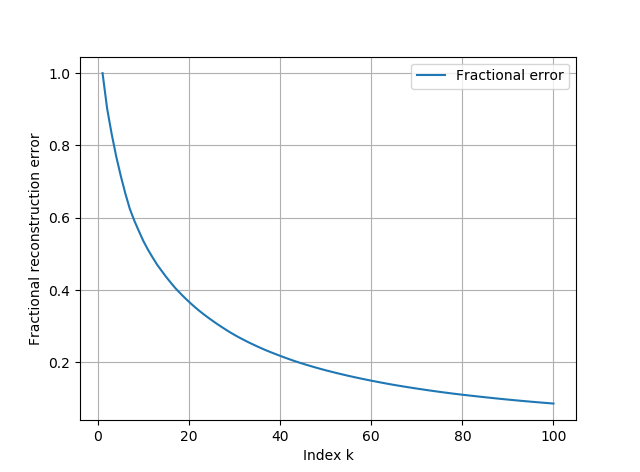
\includegraphics[width=0.66\linewidth]{../Problem_4/Problem_4.2.2.png}
	\caption{Fractional Reconstruction error for the first $k=100$ eigenvalues}
	\label{fig:4.2.2}
\end{figure}

The first $11$ eigenvalues make up $50\%$ of the total variance and the first $44$ eigenvalues make up $80\%$ of the eigenvalues. \par 
The first ten eigenvectors are shown in figure \ref{fig:4.2.4}. They should represent the dimensions with the highest variance (biggest information) and therefore should carry essential information about the ten possible digits, zero to nine.

\begin{figure}
	\centering
	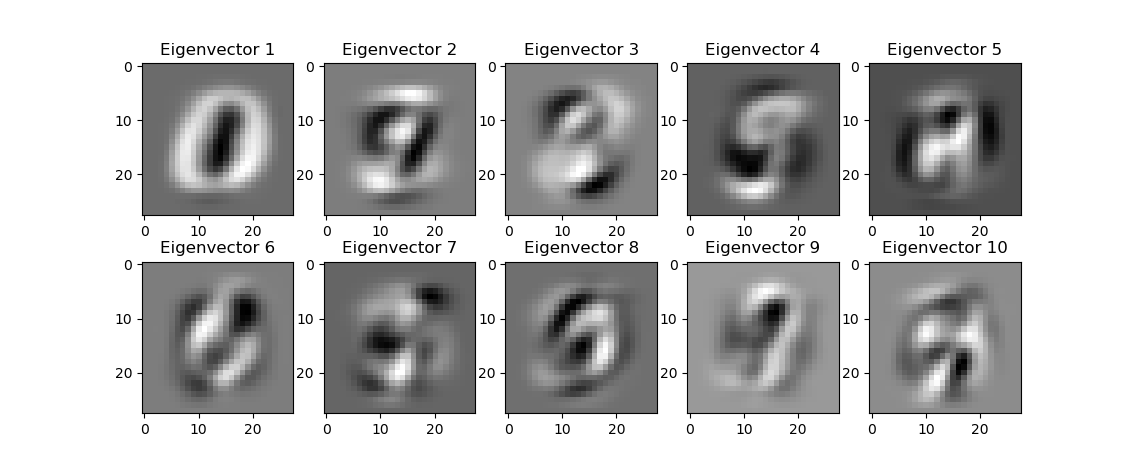
\includegraphics[width=0.66\linewidth]{../Problem_4/Problem_4.2.4.png}
	\caption{Plot of the first ten eigenvectors}
	\label{fig:4.2.4}
\end{figure}

\subsection{Pseudocode for Reconstruction}

Goal: best reconstruction (squared error should be small) for dimensionality reduction from $d$ to $k$ dimensions.
\begin{enumerate}
	\item Use the top $k$ eigenvectors since they carry the larges variance (information) for the reconstruction. The actual number $k$ is a hyperparameter which has to be optimized.
	\item By using SVD on the covariance matrix $\Sigma$ we get the $k$ eigenvalues. The top $k$ eigenvalues make up the matrix $\hat{U}\in \mathbb{R}^{d \times k}$. The reduced data matrix is then given by
	\begin{align}
	\hat{X} = \left( X - \vec{1}\cdot \vec{\mu}^T \right)\cdot \hat{U} 
	\end{align}
	\item The $d$-dimensional reconstruction is then given by
	\begin{align}
	X_\text{rec} = \hat{X}\cdot \hat{U}^T + \vec{1}\cdot\vec{\mu}
	\end{align}
\end{enumerate}

\subsection{Visualization and Reconstruction}

For $k=30$ it takes roughly $2$s to reconstruct the data. The plots are shown for different $k$ in figures \ref{fig:4.4.1} and \ref{fig:4.4.2}. For low values of $k$ ($k=1,3,5$) we can see that the reconstruction is composed of one, three and five eigenvalues. The reconstruction itself is not useful for determining the original digit. For medium $k$ ($k=10,25$) the pictures get more and more blurry until for higher $k$ ($k=50,k=200,500+$) one finally can estimate the digit for sure. It seems that the top 10 dimensions seem to capture enough information to guess the digit more or less correctly, more dimensions are better. 

\begin{figure}[h!]
	\centering
	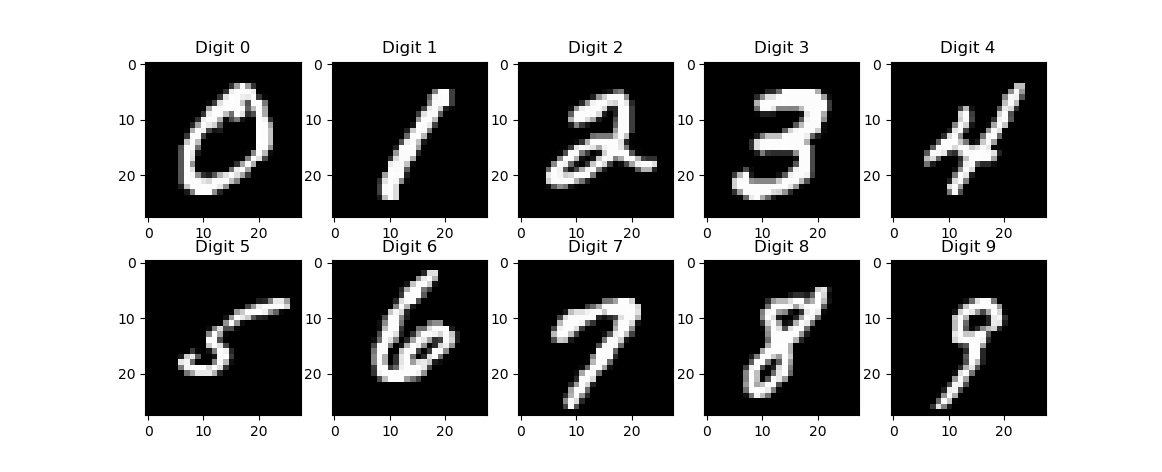
\includegraphics[width=\linewidth]{../Problem_4/Problem_4.1.1.png}
	\caption{Grey scale plot of ten digits of the MNIST database}
	\label{fig:4.1.1}
\end{figure}

\begin{figure}[h!]
	\centering
	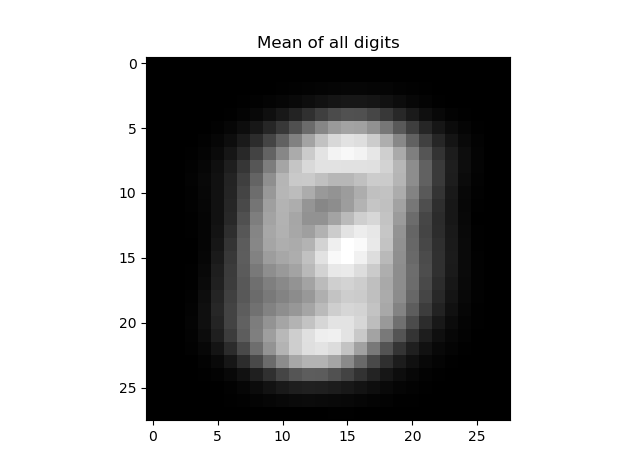
\includegraphics[width=0.66\linewidth]{../Problem_4/Problem_4.1.3_2.png}
	\caption{Grey scale plot of the mean image of the MNIST database}
	\label{fig:4.1.3}
\end{figure}

\begin{figure}[H]
	\centering
	\subfloat[Reconstruction for $k=1$] {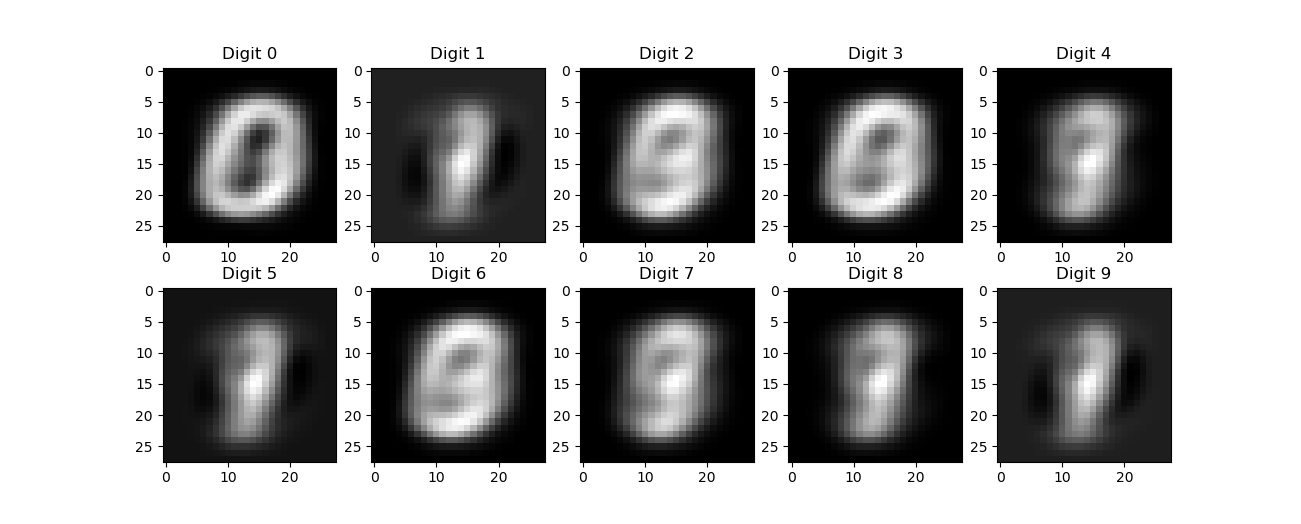
\includegraphics[width=0.49\textwidth]{../Problem_4/Problem_4.4.1.png}}
	\hfill
	\subfloat[Reconstruction for $k=3$] {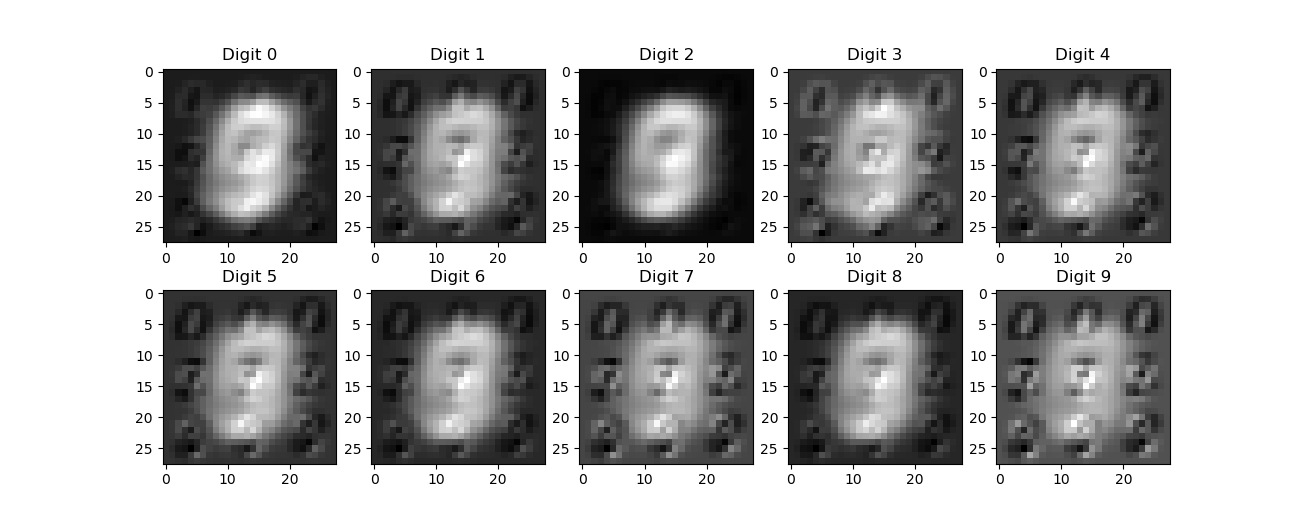
\includegraphics[width=0.49\textwidth]{../Problem_4/Problem_4.4.3.png}}
	\hfill
	\subfloat[Reconstruction for $k=5$] {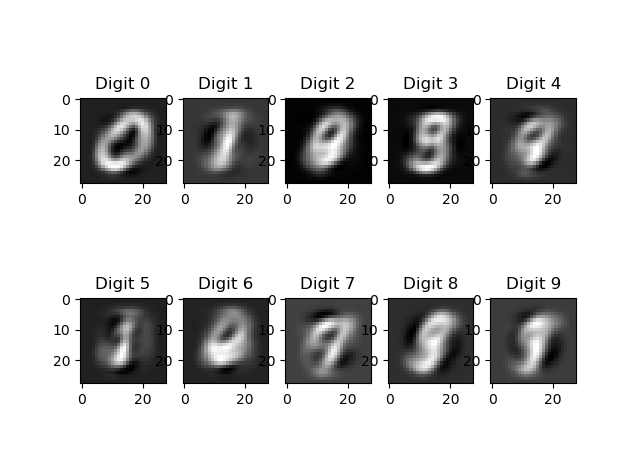
\includegraphics[width=0.49\textwidth]{../Problem_4/Problem_4.4.5.png}}
	\hfill
	\subfloat[Reconstruction for $k=10$] {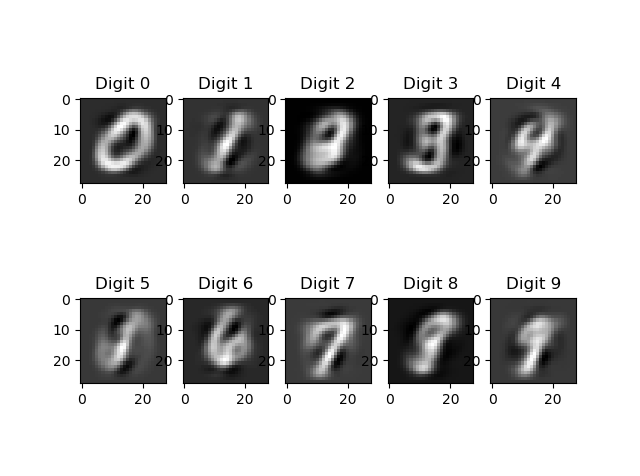
\includegraphics[width=0.49\textwidth]{../Problem_4/Problem_4.4.10.png}}
	\caption[]{Reconstruction of the ten digits used in Problem part 4.1 for different $k$.}
	\label{fig:4.4.1}
\end{figure}

\begin{figure}[H]
	\centering
	\subfloat[Reconstruction for $k=25$] {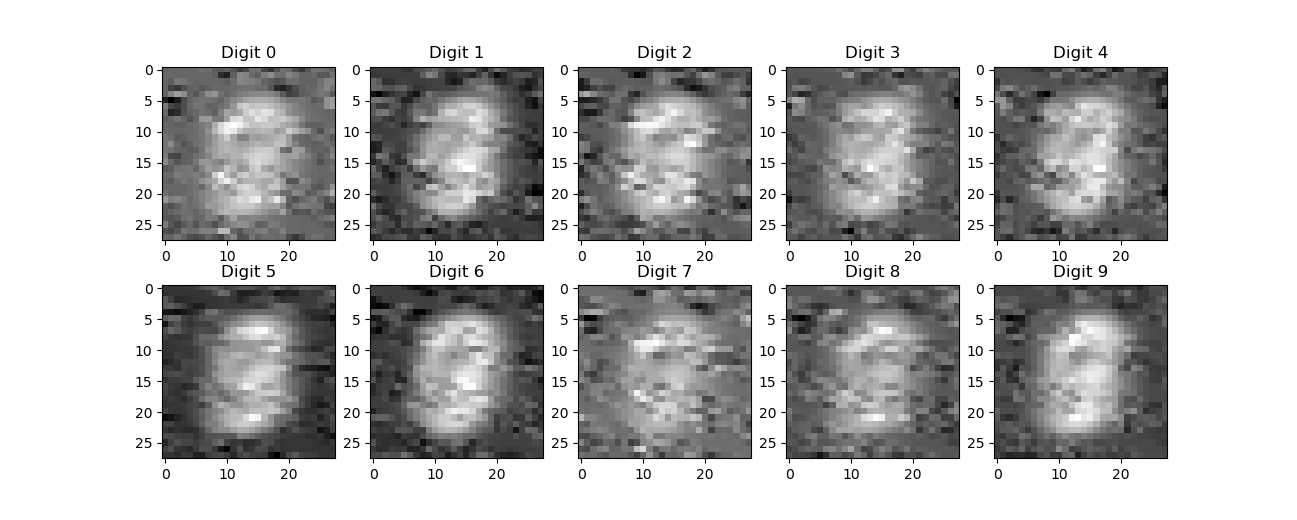
\includegraphics[width=0.49\textwidth]{../Problem_4/Problem_4.4.25.png}}
	\hfill
	\subfloat[Reconstruction for $k=50$] {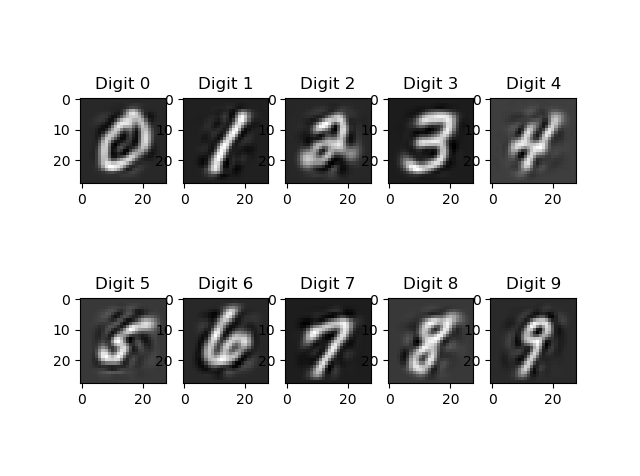
\includegraphics[width=0.49\textwidth]{../Problem_4/Problem_4.4.50.png}}
	\hfill
	\subfloat[Reconstruction for $k=200$] {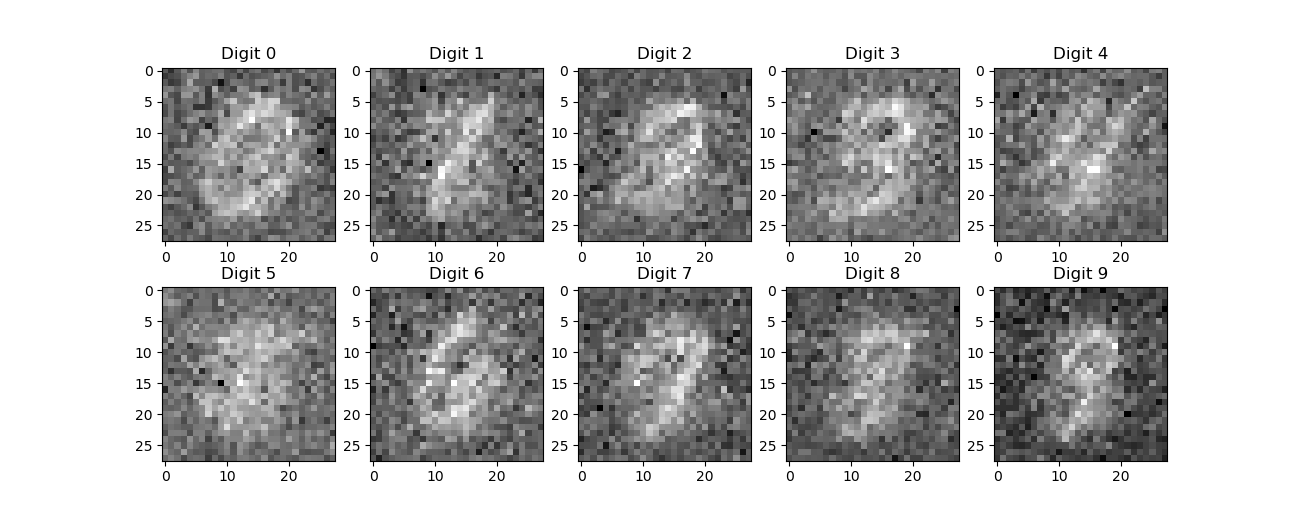
\includegraphics[width=0.49\textwidth]{../Problem_4/Problem_4.4.200.png}}
	\hfill
	\subfloat[Reconstruction for $k=500$] {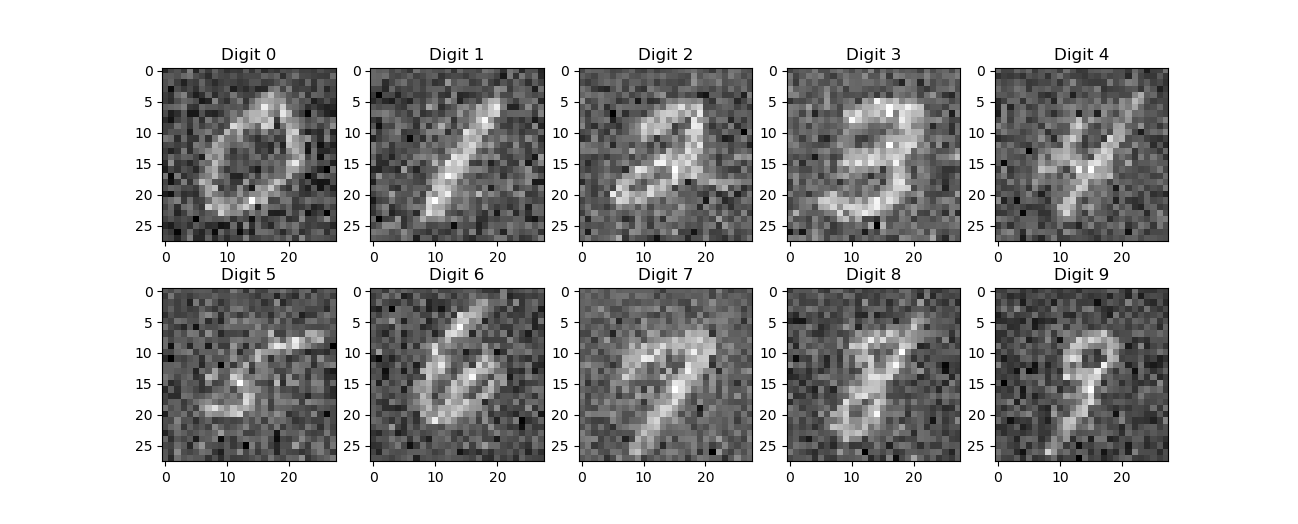
\includegraphics[width=0.49\textwidth]{../Problem_4/Problem_4.4.500.png}}
	\caption[]{Reconstruction of the ten digits used in Problem part 4.1 for different $k$. Continuation from previous page.}
	\label{fig:4.4.2}
\end{figure}

\newpage



\section{Bayes Optimal Classifier}

\begin{theorem}
	If $D$ is a distribution with samples (x,y) where x and y are independent and the theorem for the Bayesian optimal classifier holds, then the we can write
	\begin{align}
		f^{BO}(x)=\arg\max_yD(x,y) = \arg\max_yD(y|x).
	\end{align}
\end{theorem}
\begin{proof}
	When we assume that x and y are independent and the Bayesian theorem holds then we can write
	\begin{align}
		D(x,y) = D(x)D(y) = D(y)D(x|y) = D(y) \frac{D(x)}{D(y)}D(y|x) = D(x)D(y|x).
	\end{align}
	Because we want to optimize the classifier in terms of $y$ we can drop the $D(x)$ since it is a constant and independent of $y$. Therefore:
	\begin{align}
		f^{BO}(x)=\arg\max_yD(x,y) = \arg\max_yD(x)D(y|x) = \arg\max_yD(y|x)
	\end{align}
\end{proof}

This slightly different definition tries to maximize the probability to find $y$ conditioned on $x$. If we had a classifier which makes fewer errors than the Bayesian classifier then the probability to find an $y$ conditioned on $x$ would still be higher by definition for the Bayesian classifier. Therefore the overall error of BO would be smaller and the other classifier would perform worse.
\newpage

\section{Bonus: Dimensionality Reduction}

The dimensionality algorithm from previous problem was utilized to project dataset 9 down to different dimensions $k$ to test the performance. Since I expected at least two features to be noise in set 9, I though I could filter noise in form of dimensionality reduction. Plot \ref{fig:6.1} compares the performance of different $k$ for the normal perceptron implementation. One can clearly see that the performance against my expectations deteriorates. For $k=20$ we completely reconstruct the data, therefore no changes.

\begin{figure}[H]
	\centering
	\subfloat[Performance for $k=5$] {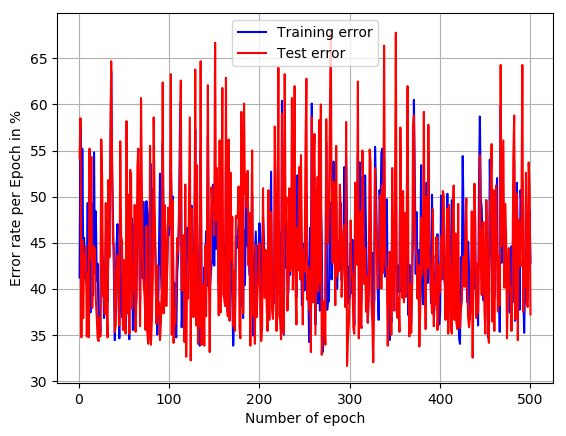
\includegraphics[width=0.25\textwidth]{../Problem_6/A2.10.train_5.tsv.full.png}}
	\hfill
	\subfloat[Performance for $k=15$] {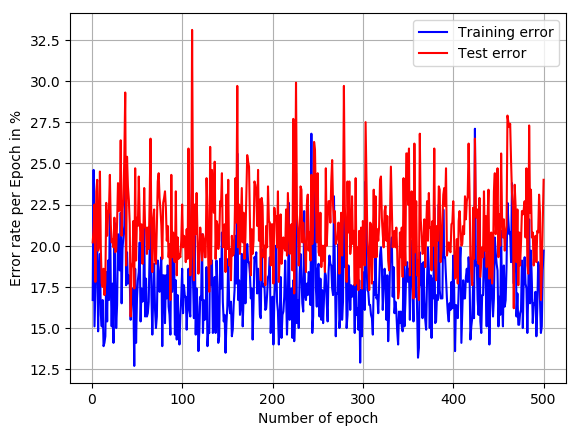
\includegraphics[width=0.25\textwidth]{../Problem_6/A2.10.train_15.tsv.full.png}}
	\hfill
	\subfloat[Performance for $k=17$] {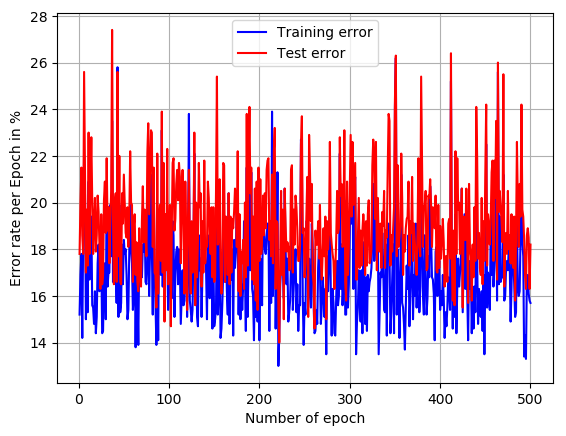
\includegraphics[width=0.25\textwidth]{../Problem_6/A2.10.train_17.tsv.full.png}}
	\hfill
	\subfloat[Performance for $k=20$] {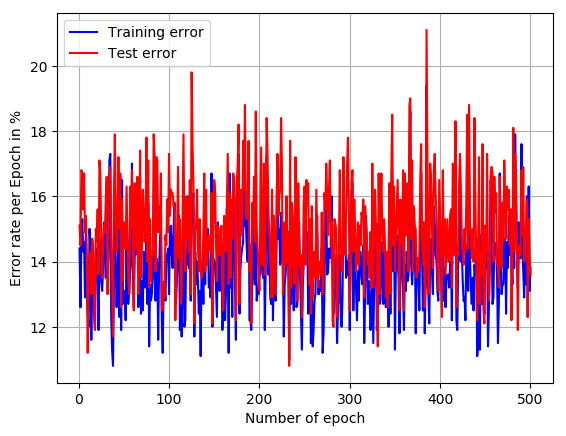
\includegraphics[width=0.25\textwidth]{../Problem_6/A2.10.train_20.tsv.full.png}}
	\caption[]{Performance for different $k$ for the normal perceptron implementation on set 9.}
	\label{fig:6.1}
\end{figure}

Since the voted perceptron has quite a long runtime I just performed only one test with $k=18$ since I expected two features to be noise, but as plot \ref{fig:6.2} shows, no improvement was yielded.

\begin{figure}[H]
	\centering
	\subfloat[Performance for $k=5$] {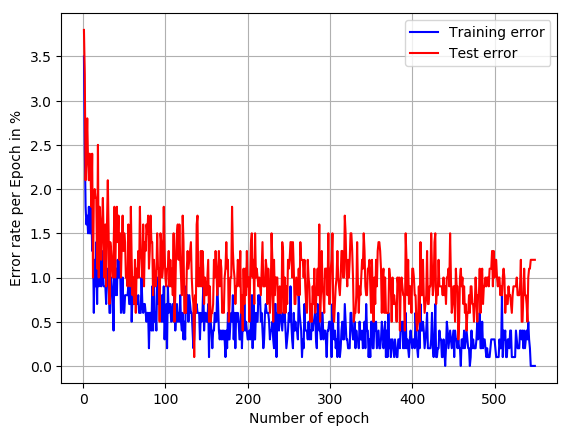
\includegraphics[width=0.3\textwidth]{../Problem_2/A2.11.train.tsv.full.png}}
	\hspace{1pt}
	\subfloat[Performance for $k=15$] {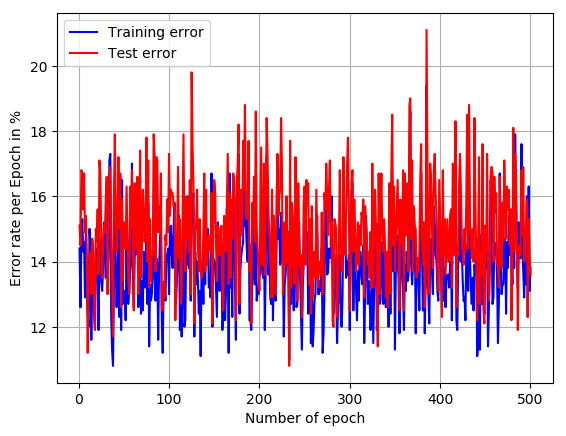
\includegraphics[width=0.3\textwidth]{../Problem_6/A2.10.train_20.tsv.full.png}}
	\caption[]{Performance for different $k=18$ for the voted perceptron implementation on set 9 (left) and the normal implementation withou dimensionality reduction (right).}
	\label{fig:6.2}
\end{figure}

%\chapter*{Bibliography}
\addcontentsline{toc}{chapter}{Bibliography}%	

\bibliographystyle{unsrt}
\bibliography{./bib}





\end{document}  